\documentclass[12pt]{article}

\usepackage{graphicx}
\usepackage[doublespacing]{setspace}
\usepackage{textcomp}
\usepackage{amsmath,bm}
\usepackage{amssymb}
\usepackage{fancyhdr}
\usepackage{lastpage}
\usepackage{float}
\usepackage{array}
\usepackage{indentfirst}
\usepackage{titletoc}
\usepackage{setspace,geometry}
\title{Optimal Transportation, Matching Problem and Hedonic Model}
\author{YuHaiyang, WangXiangtong, ZhangZhiyi, XuJiahe and WangSong}
\date{}
\begin{document}
\maketitle
\section*{0. Review of professor's problems}
Hedonic pricing is a problem in economics where buyers and sellers match together according to
their preferences to buy (respectively sell) different goods. Try to understand the mathematical
structure of this problem (it can be formulated in terms of optimal transport maps). Can the resulting
mathematical problem be given a “factories and mines” type of interpretation (hint, imagine that you
have two, rather than one, type of factory, producing say iron and aluminum, and you want to build
your mines in locations that minimize some total transport cost). Can the problem also be rewritten as
a matching (that is, pure optimal transport) problem?
\section*{1.Background}
\subsection*{1.1.Optimal Transportation Model}
\subsection*{1.2.Matching Problem Model}
\subsection*{1.3.Hedonic Price Model}
\section*{2.Our work}
\subsection*{2.1.The mathematical structure of Hedonic pricing problem}
\subsection*{2.2.Rewrite the problem as a matching problem}
\subsection*{2.3.Give a “factories and mines” type of interpretation to the resulting mathematical problem}
\section*{3.Realize the Problem}
\newpage
\section{Optimal Transportation Model}

  \subsection{Background}
    Transport theory is a name given to the study of optimal transportation and allocation of resources.  The problem was formalized by the French mathematician Gaspard Monge in 1781. Major advances were made in the field during World War II by the Soviet mathematician and economist Leonid Kantorovich. So,the problem is sometimes known as the Monge-Kantorovich transportation problem.
  \subsection{Example}

  $c: \mathbf{R}^{2}\times \mathbf{R}^{2}\rightarrow [0,\infty)$
  $$c(T):=\sum_{m\in M}c(m,T(m))$$

  \newpage
\begin{figure}
  \centering
  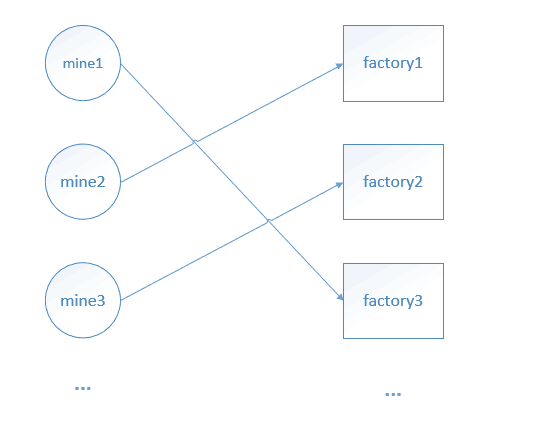
\includegraphics[width=10cm]{1.png}\\
  \caption{Mines and factories}
\end{figure}

\subsection{Abstract formulation of the problem}

Let $X$ and $Y$ be two separable metric spaces such that any probability measure on $X$ (or $Y$) is a Radon measure (i.e. they are Radon spaces). Let $c$ : $X \times Y \rightarrow [0, +\infty]$ be a Borel-measurable function. Given probability measures $\mu$ on $X$ and $\nu$ on $Y$, Monge's formulation of the optimal transportation problem is to find a transport map $T$ : $X \rightarrow Y$ that realizes the infimum
$$\mathrm{inf}\left\{ \int_{X}c(x,T(x))\ \mathrm{d}\mu(x)\Bigg| T_*(\mu)=\nu\right\} $$
where $T_*$($\mu$) denotes the push forward of $\mu$ by $T$. A map $T$ that attains this infimum (i.e. makes it a minimum instead of an infimum) is called an "optimal transport map".
\section{Matching Problem Model}
Let $X$, $Y$, and $Z$ be finite, disjoint sets, and let $T$ be a subset of $X \times Y \times Z$. That is, $T$ consists of triples $(x, y, z)$ such that $x \in X$, $y \in Y$, and $z \in Z$. Now $M \subseteq T$ is a 3-dimensional matching if the following holds: for any two distinct triples $(x_{1}, y_{1}, z_{1}) \in M $and $(x_{2}, y_{2}, z_{2}) \in M$, we have $x_{1} \neq x_{2}$, $y_{1} \neq y_{2}$, and $z_{1} \neq z_{2}$.

\section{Hedonic Price Model}
\subsection{Introduction}
Hedonic pricing is a model, which identifies price factors, according to the premise that price is determined both by internal characteristics of the good being sold and external factors affecting it.

A hedonic pricing model is often used to estimate quantitative values for ecosystem or environmental services that directly impact market prices for homes.
\subsection{Formula}
$$P=c+\sum_{n=1}^{N}\beta_{n}X_{n}+\epsilon$$

$P$: the price of house

$X_{i}$: the different characters of house

$\epsilon$: deviation

$\beta_{i}$: the coefficient of each character

$$X=(X_{1},X_{2},\ldots,X_{n})$$

\subsection{Competitive market}
To simplify the model, we suppose the market is a competitive market.
\section{Standing hypotheses of hedonic model}
To allow for the possibility that some agents choose not
to participate, we augment the spaces $X := X_{0}\cup \{\phi_{X}\}$ $Y := Y_{0}\cup \{\phi_{Y}\}$  and$
Z := Z_{0}\cup \{\phi_{Z}\}$  by including an isolated point in each: a partner $\phi_{X}$ for any
unmatched sellers, a partner ; $\phi_{Y}$ for any unmatched buyers, and the null contract $\phi_{Z}$. Preferences are encoded into functions representing the utility $u(x,z)$ of product $z\in Z$ to buyer $x\in X$, and the utility (disutility or cost) $v(y,z)$ of
product $z \in Z$ to seller $y \in Y$ . These utility functions $u : X \times Z \rightarrow R\cup \{-\infty\}$
and $v : Y \times Z \rightarrow R\cup \{+\infty\}$ are specified a priori, along with non-negative Borel measures $\mu_{0}$ on $X_{0}$ and $\nu_{0}$ on $Y_{0}$ of finite total mass representing the distribution of buyer and seller types throughout the population. The utility functions
are constrained so that neither the dummy buyer type $\phi_{X}$ nor the dummy seller
type $\phi_{Y}$ can participate in any exchange save the null contract:
\begin{equation*}
u(\phi_{X},z)=
\left\{\begin{aligned}
\quad
0&\ \ \ \text{if $z=\phi_{Z}$}\\
-\infty&\ \ \ \text{else},
\end{aligned}
\right.
\end{equation*}
\begin{equation}
u(\phi_{Y},z)=
\left\{\begin{aligned}
\quad
0&\ \ \ \text{if $z=\phi_{Z}$}\\
+\infty&\ \ \ \text{else},
\end{aligned}
\right.
\end{equation}
while the measures $\mu_{0}$ and $\nu_{0}$ are extended to $X$ and $Y$ by assigning mass
$\nu_{0}(Y_{0}) + 1$ and $\mu_{0}(X_{0}) + 1$ to the points $\phi_{X}$ and $\phi_{Y}$ respectively:
\begin{equation}
\mu:=\mu_{0} + (\nu_{0}(Y_{0}) + 1)\delta_{\phi_{X}}\ \ \ \ \nu:=\nu_{0} + (\mu_{0}(X_{0}) + 1)\delta_{\phi_{Y}}
\end{equation}
The augmented measures balance $\mu[X] = \nu[Y] < \infty$.

To guarantee the convergence of various integrals, and attainment of various suprema and infima, we assume throughout (and tacitly hereafter) that
$u(x,z) > -\infty$ extends upper semicontinuously to the completion of $X\times Z$ and
$v(y,z) < \infty$ lower semicontinuously to the completion of $Y \times Z$. We normalize
the utility of the null-contract to be zero
\begin{equation}
u(x,\phi_{Z}) = 0 = v(y,\phi_{Z})
\end{equation}
which can be achieved without loss of generality if the reserve utilities $u(x,\phi_{Z} ) \in L^{1} (X,d\mu)$ and $v(y,\phi_{Z} ) \in L^{1} (X,d\nu)$ are continuous and integrable, by subtracting them from $u$ and $v$.

Define the pairwise surplus function
\begin{equation}
s(x,y) = \underset{z\in Z}{\mathrm{sup}}\ u(x,z)-v(y,z)
\end{equation}
We assume that for each pair the supremum is attained. Further, in case $u$ or$
v$ is discontinuous or $Z$ fails to be compact, we assume the set of contracts
\begin{equation}
Z(x,y) = \mathrm{arg}\ \underset{z\in Z}{\mathrm{max}}\ u(x,z)-v(y,z)
\end{equation}
that maximize the surplus (4) is non-empty, compact, and depends upper hemicontinuously on $(x,y) \in X \times Y$. It is well-known that there exists a measurable selection, i.e., a Borel function $z_{0}:X \times Y \rightarrow Z$ such that $z_{0}(x,y)$ is
contained in $Z (x,y)$ for all $(x,y)$.

Suppose $P : Z \rightarrow \mathbf{R} \cup \{\pm\infty\}$denotes the competitive market price of quality
$z \in Z$. To allow non-participation, it is subject to the constraint $P (\phi_{Z}) = 0$.
We assume that buyer utility is linear in price so that in such a market, the
indirect utility available to buyer type $x \in X$ is defined by the quasi-linear
utility maximization
$$U(x)=\underset{z\in Z}{\mathrm{sup}} \{u(x,z)-P(z)\}$$
Here $U(x) \geq 0$ is non-negative since $\phi_{Z} \in Z$; each buyer $x$ retains the right
not to consume. Similarly, we assume seller utility is linear in price so that the
indirect utility available to seller type $y \in Y$ is given by the utility maximization
$$V(y)=\underset{z\in Z}{\mathrm{sup}} \{P(z)-v(y,z)\}$$
with $V (y) \geq 0$ and vanishing in the case of non-participation.

Let $\alpha$ be a non-negative measure on $X \times Y \times Z$. The support of $\alpha$ refers
to the smallest closed set $\mathrm{Spt}(\alpha) \subseteq X \times Y \times Z$ of full mass. The measure $\alpha$
represents an assignment of buyers and sellers to each other and to products.
We use the push-forward notation to denote its marginal projections $\pi^{X}_{\#}\alpha$ and $\pi^{Y}_{\#}\alpha$ under mappings such as
$\pi^{X}(x,y,z) = x $ and $\pi^{Y}(x,y,z) = y$ on $X \times Y\times Z$.
The pair $(\alpha,P)$ is an hedonic equilibrium if these projections coincide with
the initial measures on each set:

$$\pi^{X}_{\#}\alpha=\mu$$
$$\pi^{Y}_{\#}\alpha=\nu$$

and if, for $\alpha$-almost all points $(x,y,z) \in \mathrm{Spt} \alpha$, we have that
$$U(x)=u(x,z)-P(z)$$
$$V(y)=P(z)-v(y,z)$$
\section{The associated matching problem}
$s : X \times Y \rightarrow [0,\infty)$ is upper semicontinuous by our assumptions (3), and the
set $Z(x,y)$ where the supremum is attained (5) is non-empty, compact-valued,
and upper hemicontinuous. Our normalizations (1)-(3) permit either buyer or
seller to go unmatched (to match with a null type) and force the utility of the
unmatched state to be zero:
$$s(x,\phi_{Y})=u(x,\phi_{Z})=0$$
$$s(\phi_{X},y)=-v(\phi_{Z},y)=0$$
One can then define a pairwise matching problem by the set of $buyers$ $(X,\mu)$,
the set of $sellers$ $(Y,\nu)$, and the pairwise surplus defined by the surplus function $s$. An $assignment$ (or a $matching$) is defined as a measure $\gamma$ on $X \times Y$ , the
marginals of which coincide with $\mu$ and $\nu$. Using the same notations as above,
we thus write that
$$\pi_{X}^{\#}\gamma=\mu$$
$$\pi_{Y}^{\#}\gamma=\nu$$

where the projection mappings $\pi^{X} (x;y) = x$ and $\pi^{Y} (x;y) = y$ this time are
defined on $X \times Y$ . If $(x,y) \in (X_{0} \times Y_{0} ) \cap \mathrm{Spt}(\gamma)$, we say that $x$ and $y$ are
matched. A buyer may be matched to multiple sellers and vice versa. If $x \in X_{0}$
and there is no $y \in Y_{0}$ such that $(x,y) \in \mathrm{Spt}(\gamma)$, we say that $x$ is unmatched
(and similarly for $y$).



A payoff corresponding to $\gamma$ is a pair of functions $\overline{U}: X\rightarrow \mathbf{R}$ and $\overline{V}: Y\rightarrow \mathbf{R}$
with the normalization
$\overline{U}(\phi_{X})=0$ such that for any $(x,y)\in \mathrm{Spt}(\gamma)$
$$\overline{U}(x)+\overline{V}(y)\leq s(x,y)$$
Finally, an outcome is defined as a triple $(\gamma,\overline{U},\overline{V})$ where $(\overline{U},\overline{V})$ is a payoff corresponding to $\gamma$

\newpage
\section{Factories and mines interpretation}
\begin{figure}[!h]
  \centering
  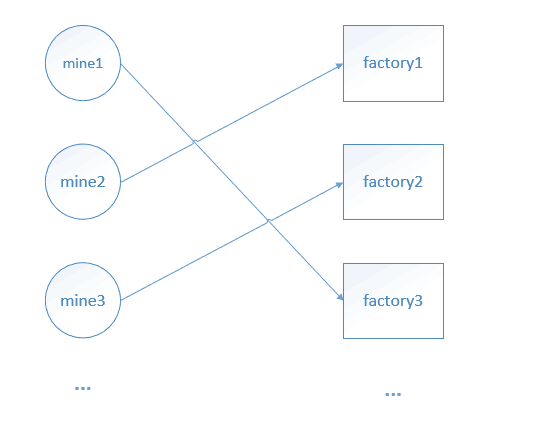
\includegraphics[width=8cm]{1.png}\\
\end{figure}

\section{How to Realize the Problem}
\subsection{}
From what above-mentioned we can simplify the problem as follow:

1.We have two sets A and B, they have the same number of elements

2.We know the cost of every connection

3.We need to find a one to one match for every element in two sets

4.The flow can be different between edges, we need to minimize the total cost
\subsection{}
Obviously this is a network problem.
As constraint conditions involve the cost of every flow and one-to-one condition, this problem can’t be solved by   The famous max-flow min-cut theorem .

By establishing an origin and a destination and making the cost of edge be the product of the flow and corresponding cost , then the problem can be solved by cost-flow algorithms.

But the time efficiency is not pleasant. Because the graph is too dense, there are too many edges on it.
\subsection{}
I found a better way to solve the problem.

As we can see, the number of elements are the same in 2 sets and besides the origin and destination, there are only 2 layers in the graph.

According to the condition: one-to-one match, we can easily remind the famous algorithm : Hungarian Algorithm

Remember, there is no cost in problems solved by Hungarian Algorithm
\subsection{}
Cardinal code in Hungarian Algorithm

\begin{figure}[H]
  \centering
  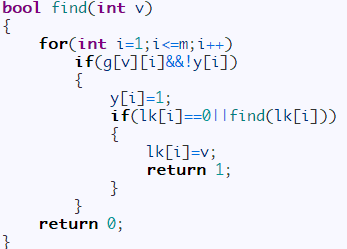
\includegraphics[width=8cm]{2.png}\\
\end{figure}

Base on the inspiration of cost-flow solution ,we only need to solve the 2-set match problem with cost on edges.

As it is quite brutal in the process of Hungarian Algorithm, we might calculate the best result in the process, but we can’t ensure it is the best solution.
\subsection{}
When we get to the best result we can easily find that:
$$\sum_{i=1}^{x_{i}\in X}lx(x_{i})+\sum_{i=1}^{y_{i}\in Y}ly(y_{i})=K=\sum weight(x_{i},y_{i})$$

$weight(a,b)$ means the cost of edge $(a,b)$

$lx(x_{i})$ means the contribution of $x_{i}$ to the whole system

$ly(y_{i})$ means the contribution of $y_{i}$ to the whole system

Also we can draw the conclusion that for every edge in the best deployment we have:
$$lx(x)+ly(y)=weight(x,y)$$
\subsection{}
In the beginning, we can only set $lx(x_{i})$ to be the max cost of edges that link to point $x_{i}$, all $ly(y_{i})$ be $0$. Then we need to adjust the value of $lx(x_{i})$ and $ly(y_{i})$ to reach the equation.

Before we reach the equation , we can easily find that
$$lx(x)+ly(y)\geq weight(x,y)$$

So the problem become that we should ensure that every element has a match and at the same time we need to adjust $lx(x_{i})$ and $ly(y_{i})$ to reach the equation.

Overall, we just need to adjust the value of $lx(x_{i})$ and $ly(y_{i})$ and then we use Hungarian algorithm to check if it is a one-to-one match. The threshold will only be decreasing. So we can make sure that the solution is the best.

\subsection{}
The strategy to reach the threshold:

We set a parameter: cnt

When we failed to get a one-to-one match
All the $lx(x_{i})$ which have a match got to minus cnt. (to decrease its contribution or importance)
To make the system be in a balance, all the $ly(y_{i})$ which have a match got to plus cnt.

We can get the best result only when the equation holds , so the set of cnt can only be the difference of the cost of edges whose end points are both be chose already.
\subsection{Cardinal code}
\begin{figure}[!h]
  \centering
  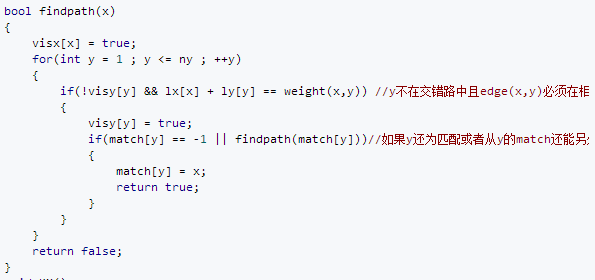
\includegraphics[width=10cm]{3.png}\\
\end{figure}

\begin{figure}[!h]
  \centering
  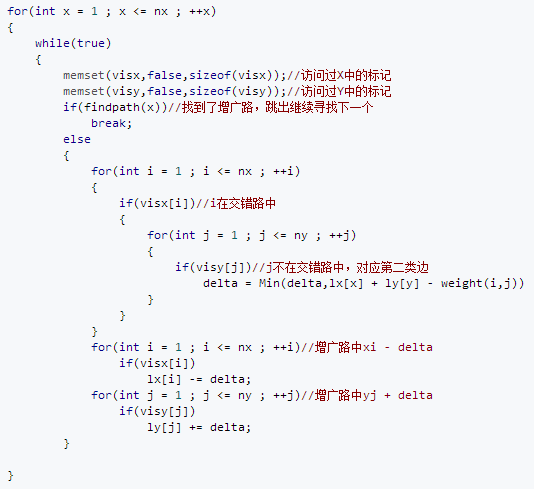
\includegraphics[width=7cm]{4.png}\\
\end{figure}
\subsection{}
By now we can find that the time cost is still quite unpleasant

Finding that there are many redundant operations in trading the graph
And the process of calculating cnt is too slow.
By using some tree structure, the process of calculating cnt can be much faster

Code : https://paste.ubuntu.com/p/BZ6ZDj7gqr/

\end{document}
